\documentclass{../../slides-style}

\slidetitle[Лекция 1: Об архитектуре]{Проектирование и архитектура ПО}{17.02.2026}

\begin{document}

    \begin{frame}[plain]
        \titlepage
    \end{frame}

    \section{Организационное}

    \begin{frame}{Организационное}
        \begin{outline}
            \1 Лекционно-практический курс, будем практиковаться по большей части прямо на парах
            \1 В конце теоретический зачёт
            \1 Балльная система ECTS
                \2 60\% за теорзачёт, 40\% за работу на парах
                \2 Прежде всего, проектирование
                    \3 Начинаем на практике -> доделываем дома -> обсуждаем на следующей практике
                    \3 -50\% баллов за пропуск дедлайна
                \2 Будут групповые и индивидуальные задания
            \1 Материалы и задания будут выкладываться в HwProj
                \2 \url{https://hwproj.ru/courses/50077}
            \1 Коммуникация в чате потока в Telegram, можно писать в личку
        \end{outline}
    \end{frame}

    \begin{frame}{Что будет в курсе}
        \begin{outline}
            \1 Объектно-ориентированное проектирование
            \1 Моделирование, язык UML и, немного, другие визуальные языки
            \1 Шаблоны проектирования и антипаттерны
            \1 Архитектурные стили
            \1 Предметно-ориентированное проектирование
            \1 Проектирование распределённых приложений
            \1 Развёртывание и DevOps
        \end{outline}
    \end{frame}

    \section{Введение}

    \begin{frame}{Программа и программный продукт}
        \begin{center}
            \includegraphics[width=0.5\textwidth]{brooksSquare.png}
        \end{center}
        \attribution{Ф. Брукс, \enquote{Мифический человеко-месяц}}
        \begin{textblock}{2}(10,-3)
            \includegraphics[width=\textwidth]{brooksCover.png}
        \end{textblock}
    \end{frame}

    \begin{frame}{Размер типичного ПО}
        \begin{footnotesize}
            \begin{center}
                \begin{tabu} {| X[0.6 l p] | X[1 l p] |}
                    \tabucline-
                    \everyrow{\tabucline-}
                    Простая игра для iOS            & 10000 LOC  \\
                    Unix v1.0 (1971)                & 10000 LOC  \\
                    Quake 3 engine                  & 310000 LOC \\
                    Windows 3.1 (1992)              & 2.5M LOC   \\
                    Linux kernel 2.6.0 (2003)       & 5.2M LOC   \\
                    MySQL                           & 12.5M LOC  \\
                    Microsoft Office (2001)         & 25M LOC    \\
                    Microsoft Office (2013)         & 45M LOC    \\
                    Microsoft Visual Studio 2012    & 50M LOC    \\
                    Windows Vista (2007)            & 50M LOC    \\
                    Mac OS X 10.4                   & 86M LOC    \\
                \end{tabu}
            \end{center}
            \url{http://www.informationisbeautiful.net/visualizations/million-lines-of-code/}
        \end{footnotesize}
    \end{frame}

    \begin{frame}{Архитектура}
        \begin{columns}
            \begin{column}{0.7\textwidth}
                \begin{outline}
                    \1 Совокупность важнейших решений об организации программной системы
                        \2 Эволюционирующий свод знаний
                        \2 Разные точки зрения
                        \2 Разный уровень детализации
                    \1 Для чего
                        \2 База для реализации, \enquote{фундамент} системы
                        \2 Инструмент для оценки трудоёмкости и отслеживания прогресса
                        \2 Средство обеспечения переиспользования
                        \2 Средство анализа системы ещё до того, как она реализована
                \end{outline}
            \end{column}
            \begin{column}{0.3\textwidth}
                \includegraphics[width=\textwidth]{whatArchitecture.png}
                \attribution{Интернеты}
            \end{column}
        \end{columns}
    \end{frame}

    \section{Профессия \enquote{Архитектор}}

    \begin{frame}{Профессия \enquote{Архитектор}}
        \begin{outline}
            \1 Архитектор --- специально выделенный человек (или группа людей), отвечающий за:
                \2 разработку и описание архитектуры системы
                \2 доведение её до всех заинтересованных лиц
                \2 контроль реализации архитектуры
                \2 поддержание её актуального состояния по ходу разработки и сопровождения
        \end{outline}
    \end{frame}

    \begin{frame}{Трудовые функции архитектора}
        \framesubtitle{По профстандарту 06.003}
        \begin{outline}
            \1 Выявление и согласование требований к программной системе с точки зрения архитектуры
            \1 Выбор и моделирование архитектурного решения для реализации программной системы
            \1 Разработка разделов по архитектуре проектных и эксплуатационных документов программной системы
            \1 Контроль реализации и испытаний программной системы с точки зрения архитектуры
            \1 Сопровождение эксплуатации программной системы с точки зрения архитектуры
        \end{outline}
    \end{frame}

    \begin{frame}{Архитектор vs разработчик}
        \begin{center}
            \includegraphics[width=0.35\textwidth]{architectVsDeveloper.png}
        \end{center}
        \begin{outline}
            \1 Широта знаний
            \1 Коммуникационные навыки
            \1 Часто архитектор играет роль разработчика и наоборот
                \2 Архитектор в \enquote{башне из слоновой кости} --- это плохо
        \end{outline}
    \end{frame}

    \section{Пример: ПО для осциллографа}

    \begin{frame}{Пример: ПО для осциллографа}
        \begin{columns}
            \begin{column}{0.6\textwidth}
                \begin{outline}
                    \1 Считывать параметры сигнала
                    \1 Оцифровывать и сохранять их
                    \1 Выполнять разные фильтрации и преобразования
                    \1 Отображать результаты на экране
                        \2 С тач-скрином и встроенным хелпом
                    \1 Возможность настройки под конкретные задачи
                \end{outline}
            \end{column}
            \begin{column}{0.4\textwidth}
                \begin{center}
                    \includegraphics[width=0.9\textwidth]{oscilloscope.png}
                \end{center}
                \attribution{Hantek}
            \end{column}
        \end{columns}
        \vspace{1cm}
        \begin{tiny}
            По статье Garlan D., Shaw M. An introduction to software architecture
        \end{tiny}
    \end{frame}

    \begin{frame}{Вариант 1: объектная модель}
        \begin{center}
            \includegraphics[width=0.5\textwidth]{oscilloscopeObjects.png}
            \attribution{Garlan D., Shaw M. An introduction to software architecture}
        \end{center}
    \end{frame}

    \begin{frame}{Вариант 2: слоистая архитектура}
        \begin{center}
            \includegraphics[width=0.5\textwidth]{oscilloscopeLayers.png}
            \attribution{Garlan D., Shaw M. An introduction to software architecture}
        \end{center}
    \end{frame}

    \begin{frame}{Вариант 3: каналы и фильтры}
        \begin{center}
            \includegraphics[width=0.5\textwidth]{oscilloscopeFilters.png}
            \attribution{Garlan D., Shaw M. An introduction to software architecture}
        \end{center}
    \end{frame}

    \begin{frame}{Вариант 4: модифицированные каналы и фильтры}
        \begin{center}
            \includegraphics[width=0.5\textwidth]{oscilloscopeModifiedFilters.png}
            \attribution{Garlan D., Shaw M. An introduction to software architecture}
        \end{center}
    \end{frame}

    \begin{frame}{Выводы}
        \begin{outline}
            \1 Можем делать утверждения о свойствах системы, базируясь на её структурных свойствах
                \2 Не написав ни строчки кода и даже не выбрав язык реализации
            \1 Рассуждения очень субъективны
                \2 Многое зависит от интуиции и вкуса архитектора, однако ошибки очень дороги
            \1 Можно выделить \emph{архитектурные стили} --- \enquote{архитектуры архитектур}
            \1 Можно выделить \emph{архитектурные точки зрения} и \emph{архитектурные виды}
            \1 Разный уровень детализации
        \end{outline}
    \end{frame}

    \section{Архитектурные виды}

    \begin{frame}{Архитектурные виды}
        \framesubtitle{Стандарт IEEE 1016-2009}
        \begin{outline}
            \1 Контекст --- фиксирует окружение системы
                \2 Диаграммы активностей UML, IDEF0 (SADT)
            \1 Композиция --- описывает крупные части системы и их предназначение
                \2 Диаграммы компонентов UML, IDEF0
            \1 Логическая структура --- структура системы в терминах классов, интерфейсов и отношений между ними
                \2 Диаграммы классов UML, диаграммы объектов UML
        \end{outline}
    \end{frame}

    \begin{frame}{Архитектурные виды (2)}
        \begin{outline}
            \1 Зависимости --- определяет связи по данным между элементами
                \2 Диаграммы компонентов UML, диаграммы пакетов UML
            \1 Информационная структура --- определяет персистентные данные в системе
                \2 Диаграммы классов UML, IDEF1x, ER, ORM
            \1 Использование шаблонов --- документирование использования локальных паттернов проектирования
                \2 Диаграммы классов UML, диаграммы пакетов UML, диаграммы коллабораций UML
        \end{outline}
    \end{frame}

    \begin{frame}{Архитектурные виды (3)}
        \begin{outline}
            \1 Интерфейсы --- специфицирует информацию о внешних и внутренних интерфейсах
                \2 IDL, диаграммы компонентов UML, макеты пользовательского интерфейса, неформальные описания сценариев использования
            \1 Структура системы --- рекурсивное описание внутренней структуры компонентов системы
                \2 Диаграммы композитных структур UML, диаграммы классов UML, диаграммы пакетов UML
            \1 Взаимодействия --- описывает взаимодействие между сущностями
                \2 Диаграммы композитных структур UML, диаграммы взаимодействия UML, диаграммы последовательностей UML
        \end{outline}
    \end{frame}

    \begin{frame}{Архитектурные виды (4)}
        \begin{outline}
            \1 Динамика состояний --- описание состояний и правил переходов между состояниями
                \2 Диаграммы конечных автоматов UML, диаграммы Харела, сети Петри
            \1 Алгоритмы --- описывает в деталях поведение каждой сущности
                \2 Диаграммы активностей UML, псевдокод, настоящие языки программирования
            \1 Ресурсы --- описывает использование внешних ресурсов
                \2 Диаграммы развёртывания UML, диаграммы классов UML, OCL
        \end{outline}
    \end{frame}

    \begin{frame}{Ещё про архитектурные виды}
        \begin{outline}
            \1 Пример --- \url{http://robotics.ee.uwa.edu.au/courses/design/examples/example_design.pdf}
            \1 Ни один вид не обязателен
            \1 Активно используются визуальные языки
                \2 В основном как дополнение к тексту
            \1 Моделирование принципиально важно для архитектуры
                \2 Нельзя абстрагироваться от сложности, но можно декомпозировать сложность
        \end{outline}
    \end{frame}

    \section{Роль архитектуры в жизненном цикле}

    \begin{frame}{Роль архитектуры в жизненном цикле}
        \begin{center}
            \includegraphics[width=0.5\textwidth]{architectureLifeCycle.png}
            \attribution{Z. Quin, ``Software Architecture''}
        \end{center}
    \end{frame}

    \begin{frame}{Архитектура и требования}
        \begin{center}
            \includegraphics[width=0.8\textwidth]{useCaseDiagram.png}
        \end{center}
    \end{frame}

    \begin{frame}{Требования}
        \begin{outline}
            \1 Функциональные --- то, \emph{что} система должна делать
            \1 Нефункциональные --- то, \emph{как} система должна это делать
                \2 Эффективность
                \2 Масштабируемость
                \2 Удобство использования
                \2 Надёжность
                \2 Безопасность
                \2 Сопровождаемость и расширяемость
                \2 ...
            \1 Ограничения
                \2 Технические
                \2 Бизнес-ограничения
        \end{outline}
    \end{frame}

    \begin{frame}{Архитектура и проектирование}
        \begin{center}
            \includegraphics[width=0.9\textwidth]{trikRuntimeComponents.png}
        \end{center}
    \end{frame}

    \begin{frame}{Архитектура и проектирование --- задачи}
        \begin{outline}
            \1 Декомпозиция задачи
            \1 Определение границ компонентов
            \1 Определение интерфейсов между компонентами
            \1 Общие для всей системы вопросы
                \2 Стратегия обработки ошибок
                \2 Стратегия логирования
                \2 Стратегия обновлений
                \2 Стратегия разделения доступа
                \2 Вопросы локализации
                \2 ...
            \1 Анализ и верификация архитектуры
        \end{outline}
    \end{frame}

    \begin{frame}{Архитектура и разработка}
        \begin{outline}
            \1 \emph{prescriptive architecture} --- архитектура, как её определил архитектор
            \1 \emph{descriptive architecture} --- архитектура, как она есть в системе
                \2 Архитектура у ПО есть всегда, как вес у камня
            \1 \emph{architectural drift} --- \enquote{сползание} фактической архитектуры
                \2 появление в ней важных решений, которых нет в описательной архитектуре
            \1 \emph{architectural erosion} --- \enquote{размывание} архитектуры
                \2 отклонения от описательной архитектуры, нарушения ограничений
            \1 Антипаттерн \enquote{\emph{Big ball of mud}} --- результат эрозии
        \end{outline}
    \end{frame}

    \section{Пример: Hadoop}

    \begin{frame}{Пример: Hadoop}
        \framesubtitle{As-designed}
        \begin{center}
            \includegraphics[width=0.6\textwidth]{hadoopPrescriptive.png}
        \end{center}
        \begin{scriptsize}\textcolor{gray}{Special thanks to prof. Nenad Medvidovic (USC) for kind permission for using his slides}\end{scriptsize}
    \end{frame}

    \begin{frame}{Hadoop as-built}
        \framesubtitle{HDFS}
        \begin{center}
            \includegraphics[width=0.9\textwidth]{hadoopDescriptive.png}
            \attribution{Nenad Medvidovic}
        \end{center}
    \end{frame}

    \begin{frame}{Hadoop as-built}
        \framesubtitle{HDFS + MapReduce}
        \begin{center}
            \includegraphics[width=0.7\textwidth]{hdfsMapReduce.png}
            \attribution{Nenad Medvidovic}
        \end{center}
    \end{frame}

    \begin{frame}{Hadoop as-built}
        \framesubtitle{Полная архитектура}
        \begin{center}
            \includegraphics[width=0.9\textwidth]{hadoopFull.png}
            \attribution{Nenad Medvidovic}
        \end{center}
    \end{frame}

    \begin{frame}{Hadoop as-built}
        \framesubtitle{Граф зависимостей}
        \begin{center}
            \includegraphics[width=0.5\textwidth]{hadoopDependencies.png}
            \attribution{Nenad Medvidovic}
        \end{center}
    \end{frame}

\end{document}
